\documentclass[chaptersright]{informeutn}

% Paquetes adicionales requeridos que no están en la clase base
\usepackage{csquotes}
\usepackage[backend=bibtex, style=alphabetic, sorting=ynt]{biblatex}
\addbibresource{fuentes.bib}
\usepackage{siunitx}
\usepackage{circuitikz}
\usetikzlibrary{arrows, arrows.meta, positioning, shapes.geometric}
\usepackage{subcaption}
\usepackage{listings}
\usepackage{hyperref}

% Definición de estilo para código
\lstdefinestyle{customcode}{
  backgroundcolor=\color{gray!10},
  basicstyle=\ttfamily\small,
  keywordstyle=\color{blue},
  frame=single,
  breaklines=true,
  captionpos=b
}
\lstset{style=customcode}

% Metadatos del Documento
\materia{EA2, TD2, MEIE}
\titulo{Control Numerico Computalizado}
\subtitulo{Anteproyecto}
\comision{4R2}
\autores{
    Gil, Ignacio - 401891 (sólo Electrónica Aplicada II)\\
    Grasso, Gaston - 401892\\
    Palombo, Franco - 401910\\
    Prieto, Angelo - 401012
}
\fecha{\today}

\begin{document}

\maketitle

\tableofcontents
\setcounter{page}{1}
\thispagestyle{plain}

\chapter{Introducción y Objetivos del Anteproyecto}
\label{sec:introduccion}

El presente anteproyecto documenta la propuesta para el Trabajo Integrador correspondiente al cuarto año de la
carrera de Ingeniería Electrónica en la Universidad Tecnológica Nacional, Facultad Regional Córdoba (UTN-FRC).
El objetivo central consiste en el diseño, desarrollo y validación experimental de una máquina de control numérico
computarizado (CNC) de tres ejes (X, Y, Z), orientada a aplicaciones de fresado ligero y prototipado rápido de
circuitos impresos (PCB).

Una particularidad tecnológica del proyecto reside en la reutilización sustentable de la estructura mecánica y
elementos de transmisión (guías lineales, husillos y chasis de soporte) provenientes de impresoras fuera de uso.
Esta aproximación fomenta la economía circular y plantea un desafío de ingeniería electromecánica: adaptar sistemas
de potencia y control a mecánicas heterogéneas no estandarizadas.

\section{Integración Académica Interdisciplinaria}
\label{sec:integracion}

El trabajo integrador articula los conocimientos teóricos y prácticos adquiridos en tres asignaturas clave del
nivel:

\begin{itemize}
  \item \textbf{Electrónica Aplicada II:} Implementación de etapas analógicas de acondicionamiento de señal, sensado
    de corriente en derivadores (\textit{shunts}) mediante amplificadores operacionales y detección comparada de
    sobrecorriente para actuar como final de carrera electrónico inteligente (detección de atascamiento o
    \textit{stall detection}).
  \item \textbf{Técnicas Digitales II:} Diseño e implementación de la arquitectura del sistema embebido bajo el
    sistema operativo en tiempo real FreeRTOS, desarrollo del módulo interpretador de comandos de código G (G-code),
    gestión de periféricos de comunicación (SPI, I2C, UART), temporizadores por hardware para generación de impulsos y
    diseño de la interfaz hombre-máquina (HMI) local.
  \item \textbf{Máquinas e Instalaciones Eléctricas:} Diseño y dimensionamiento de los controladores de potencia
    modulares (un canal independiente por eje) para motores paso a paso bipolares/unipolares (control de velocidad,
    dirección y evaluación de micropasos por troceado) y del controlador de potencia PWM para el motor DC de la fresa
    (\textit{spindle}).
\end{itemize}

\section{Campos de Aplicación}
\label{sec:aplicacion}

La plataforma desarrollada posee aplicaciones concretas en diversos ámbitos:
\begin{enumerate}
  \item Prototipado rápido de placas de circuito impreso mediante ruteado directo por aislamiento (PCB milling).
  \item Grabado y mecanizado liviano de materiales no ferrosos (madera, acrílico, MDF, placas FR4).
  \item Plataforma didáctica modular para la experimentación en control de movimiento, robótica y sistemas en tiempo
    real.
\end{enumerate}

\section{Arquitectura General del Sistema}
\label{sec:bloques_general}

El sistema global se estructura mediante una arquitectura modular distribuida en bloques funcionales, tal como se
esquematiza en la figura~\ref{fig.ej1:bloques_general}.

\begin{figure}[!ht]
  \centering
  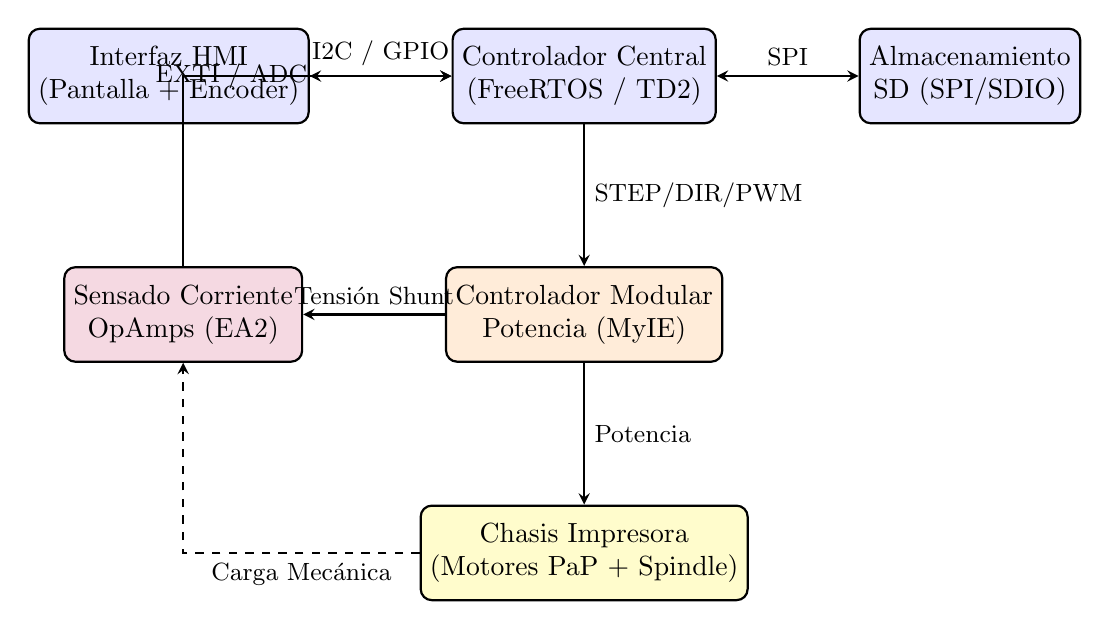
\begin{tikzpicture}[node distance=1.8cm and 1.8cm, >=stealth, thick,
  block/.style={draw, fill=blue!10, rectangle, minimum height=1.2cm, minimum width=2.8cm, text centered, rounded corners, align=center},
  powerblock/.style={draw, fill=orange!15, rectangle, minimum height=1.2cm, minimum width=2.8cm, text centered, rounded corners, align=center},
  sensorblock/.style={draw, fill=purple!15, rectangle, minimum height=1.2cm, minimum width=2.8cm, text centered, rounded corners, align=center},
  mechblock/.style={draw, fill=yellow!20, rectangle, minimum height=1.2cm, minimum width=2.8cm, text centered, rounded corners, align=center}]

  % Nodos de la fila superior (Control y HMI)
  \node [block] (mcu) {Controlador Central \\ (FreeRTOS / TD2)};
  \node [block, left=of mcu] (hmi) {Interfaz HMI \\ (Pantalla + Encoder)};
  \node [block, right=of mcu] (storage) {Almacenamiento \\ SD (SPI/SDIO)};

  % Nodos de la fila intermedia y inferior
  \node [powerblock, below=of mcu] (driver) {Controlador Modular \\ Potencia (MyIE)};
  \node [sensorblock, left=of driver] (opamp) {Sensado Corriente \\ OpAmps (EA2)};
  \node [mechblock, below=of driver] (cnc) {Chasis Impresora \\ (Motores PaP + Spindle)};

  % Conexiones superiores
  \draw [<->] (hmi) -- node[above, font=\small] {I2C / GPIO} (mcu);
  \draw [<->] (storage) -- node[above, font=\small] {SPI} (mcu);

  % Conexiones de potencia y sensado
  \draw [->] (mcu) -- node[right, font=\small] {STEP/DIR/PWM} (driver);
  \draw [->] (driver) -- node[above, font=\small] {Tensión Shunt} (opamp);
  \draw [->] (driver) -- node[right, font=\small] {Potencia} (cnc);

  % Retornos y realimentación (Líneas ortogonales)
  \draw [->] (opamp) |- node[near end, left, font=\small] {EXTI / ADC} (mcu);
  \draw [->, dashed] (cnc) -| node[near start, below, font=\small] {Carga Mecánica} (opamp);
\end{tikzpicture}

  \caption{Diagrama en bloques general del sistema CNC modular y su articulación por asignatura.}
  \label{fig.ej1:bloques_general}
\end{figure}

El controlador central ejecuta FreeRTOS y se encarga de recibir las instrucciones, calcular trayectorias y emitir las
señales de control hacia los módulos de potencia. Cada canal de potencia acciona la máquina eléctrica correspondiente y
ofrece un punto de muestreo para que la etapa de acondicionamiento analógico supervise el consumo de corriente en todo
momento.

\chapter{Electrónica Aplicada II: Sensado de Corriente y Finales de Carrera Electrónicos}
\label{sec:electronica_aplicada_2}

En el marco de la asignatura Electrónica Aplicada II, el proyecto aborda el diseño de una etapa analógica de alta
precisión para la medición continua de corriente en los motores de accionamiento y la detección electrónica de topes
mecánicos (\textit{stall detection}).

\section{Justificación Técnica y Objetivos del Módulo Analógico}
\label{sec:ea2_objetivos}

Los sistemas CNC convencionales emplean interruptores electromecánicos o sensores ópticos como finales de carrera en
los extremos de cada eje. En el presente proyecto, con el propósito de maximizar el aprovechamiento de los conceptos
de amplificadores operacionales y procesamiento analógico de señales, se implementa un sistema de final de carrera
electrónico basado en la detección del incremento severo de corriente cuando un eje alcanza su límite físico o sufre
un atascamiento mecánico.

El módulo analógico debe cumplir con las siguientes funciones primarias:
\begin{itemize}
  \item Muestreo de la caída de tensión en una resistencia de valor muy bajo ($R_{shunt}$) ubicada en la rama de retorno
    de cada canal del controlador de potencia.
  \item Amplificación diferencial con rechazo en modo común para eliminar el ruido provocado por las conmutaciones de
    potencia.
  \item Filtrado pasa-bajos para atenuar componentes armónicas de alta frecuencia generadas por la modulación por ancho
    de pulso (PWM).
  \item Acondicionamiento de señal con doble salida: una señal analógica continua proporcional a la corriente del
    motor dirigida al conversor analógico-digital (ADC) y una salida digital producida por un comparador con
    histéresis para disparo inmediato de interrupción.
\end{itemize}

\section{Diseño del Circuito de Sensado con Amplificadores Operacionales}
\label{sec:ea2_circuito}

En la figura~\ref{crkt.ej2:sensado_opamp} se ilustra el esquema eléctrico propuesto para la etapa de acondicionamiento.
La tensión en extremos de la resistencia derivadora $R_{shunt}$ es tomada por un amplificador operacional en
configuración diferencial.

\begin{figure}[!ht]
  \centering
  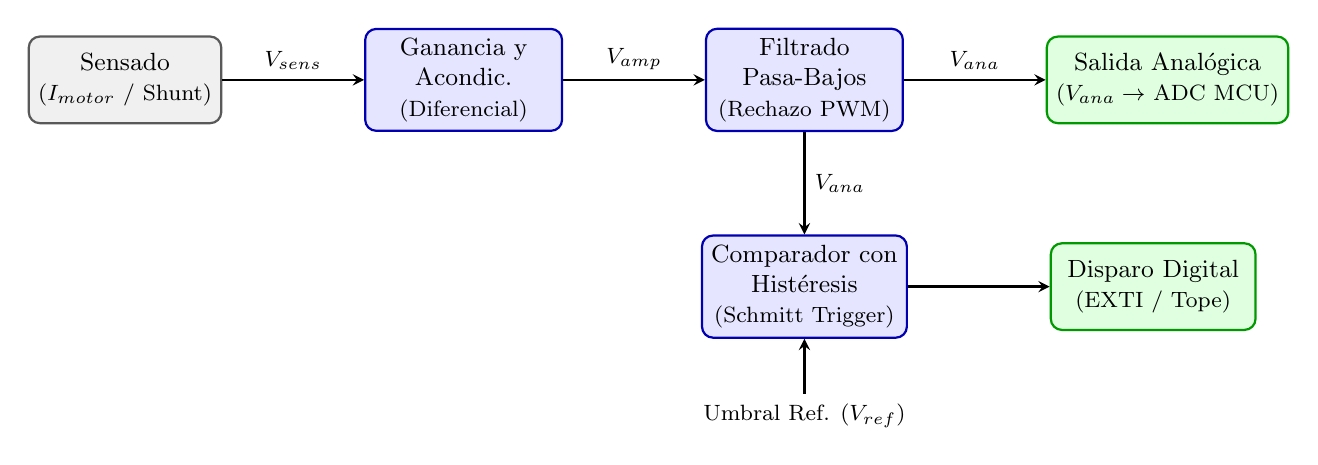
\begin{tikzpicture}[
  >=stealth, thick,
  font=\small,
  node distance=1.2cm and 1.8cm,
  block/.style={draw=blue!70!black, fill=blue!10, rectangle, rounded corners=4pt, minimum height=1.1cm, minimum width=2.5cm, align=center},
  inputnode/.style={draw=gray!70!black, fill=gray!12, rectangle, rounded corners=4pt, minimum height=1.1cm, minimum width=2.4cm, align=center},
  outnode/.style={draw=green!60!black, fill=green!12, rectangle, rounded corners=4pt, minimum height=1.1cm, minimum width=2.6cm, align=center}
]

  % Fila 1: Cadena Analógica Principal
  \node[inputnode] (trans) {Sensado\\{\footnotesize ($I_{motor}$ / Shunt)}};
  \node[block, right=of trans] (amp) {Ganancia y\\Acondic.\\{\footnotesize (Diferencial)}};
  \node[block, right=of amp] (filtro) {Filtrado\\Pasa-Bajos\\{\footnotesize (Rechazo PWM)}};
  \node[outnode, right=of filtro] (adc) {Salida Analógica\\{\footnotesize ($V_{ana} \rightarrow$ ADC MCU)}};

  % Fila 2: Etapa de Comparación y Disparo
  \node[block, below=1.3cm of filtro] (comp) {Comparador con\\Histéresis\\{\footnotesize (Schmitt Trigger)}};
  \node[outnode, right=of comp] (exti) {Disparo Digital\\{\footnotesize (EXTI / Tope)}};

  % Conexiones Horizontales con etiquetas arriba
  \draw[->] (trans) -- node[above, font=\footnotesize] {$V_{sens}$} (amp);
  \draw[->] (amp) -- node[above, font=\footnotesize] {$V_{amp}$} (filtro);
  \draw[->] (filtro) -- node[above, font=\footnotesize] {$V_{ana}$} (adc);

  % Conexión vertical directa hacia la etapa comparadora
  \draw[->] (filtro) -- node[right, font=\footnotesize] {$V_{ana}$} (comp);
  \draw[->] (comp) -- (exti);

  % Entrada de umbral de referencia
  \draw[<-] (comp.south) -- ++(0,-0.7) node[below, font=\footnotesize] {Umbral Ref. ($V_{ref}$)};

\end{tikzpicture}

  \caption{Esquema circuital de sensado de corriente con amplificador diferencial, filtro RC y comparador Schmitt.}
  \label{crkt.ej2:sensado_opamp}
\end{figure}

La relación de transferencia teórica para la etapa amplificadora diferencial está dada por la ecuación~\ref{eq.ej2:vo_diff}:

\begin{equation}
  V_{diff} = \left( \frac{R_f}{R_1} \right) \cdot I_{motor} \cdot R_{shunt}
  \label{eq.ej2:vo_diff}
\end{equation}

Donde $R_f / R_1$ establece la ganancia de tensión ($A_v$) requerida para escalar la militensión en el shunt hacia el
rango dinámico del ADC del microcontrolador ($0\V$ a $3.3\V$).

\section{Filtrado y Detector de Umbral con Histéresis (Schmitt Trigger)}
\label{sec:ea2_schmitt}

La corriente en los devanados del motor presenta rizo debido a la conmutación de los transistores del driver. Para
evitar falsos disparos en el detector de límite, la señal amplificada atraviesa un filtro pasa-bajos pasivo de primer
orden ($R_{flt}, C_{flt}$) cuya frecuencia de corte se define en la ecuación~\ref{eq.ej2:fc_filter}:

\begin{equation}
  f_c = \frac{1}{2 \pi \cdot R_{flt} \cdot C_{flt}}
  \label{eq.ej2:fc_filter}
\end{equation}

La señal filtrada $V_{ana}$ se aplica a la entrada inversora de un comparador configurado con histéresis no inversora o
inversora (disparador Schmitt). El umbral de referencia $V_{ref}$ se ajusta mediante un divisor resistivo con
potenciómetro, fijando el nivel de corriente equivalente al atascamiento físico del cabezal.

Cuando $V_{ana}$ supera a $V_{ref}$, la salida del comparador conmuta de estado lógico alto a bajo, generando una
transición limpia requerida por los pines de interrupción del controlador. La histéresis añadida mediante $R_{h1}$ y
$R_{h2}$ previene la oscilación indeseada en la zona de transición.

\section{Flujo de Operación del Sensado}
\label{sec:ea2_flujo}

La figura~\ref{fig.ej2:flujo_sensado} representa el algoritmo analógico-digital de supervisión de la corriente de los
motores.

\begin{figure}[!ht]
  \centering
  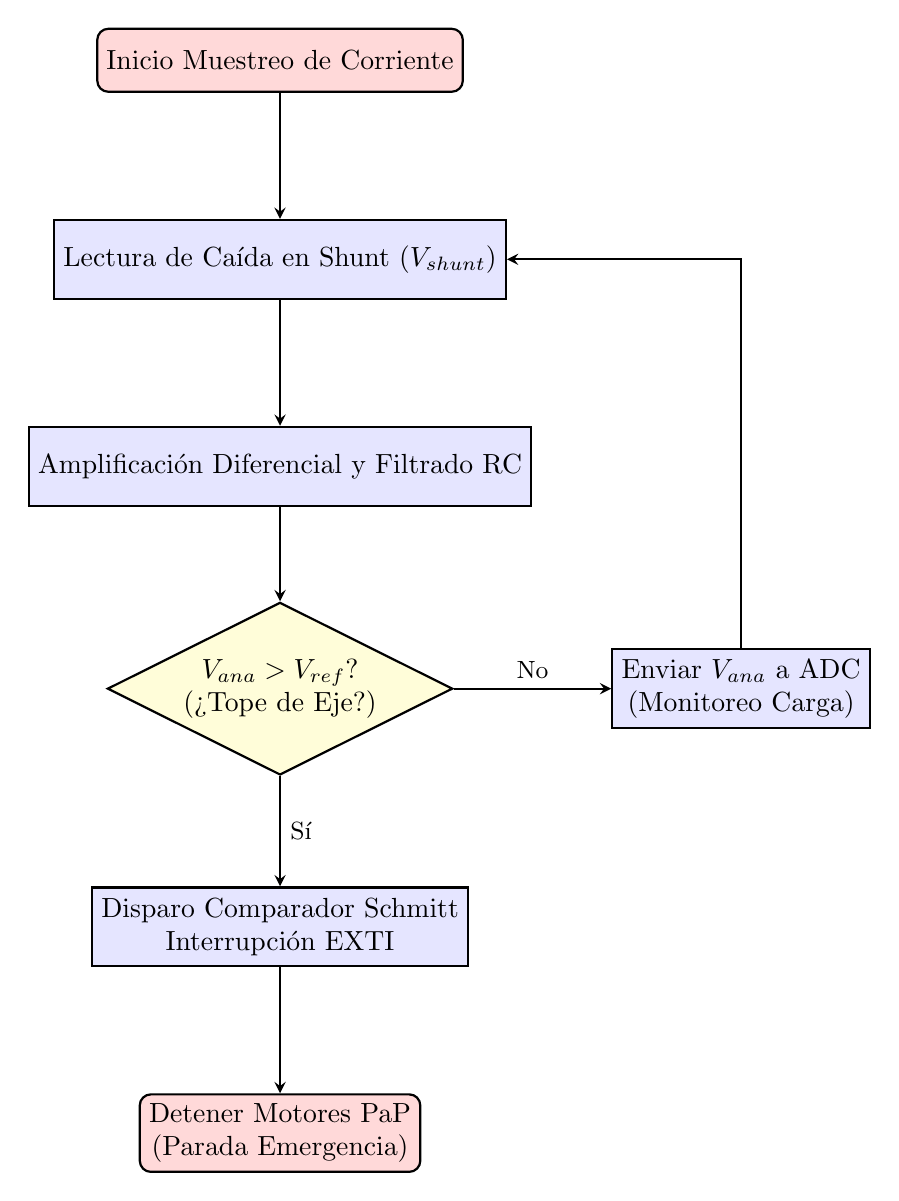
\begin{tikzpicture}[node distance=1.6cm, auto, >=stealth, thick,
  startstop/.style={draw, fill=red!15, rectangle, rounded corners, minimum height=0.8cm, text centered, align=center},
  process/.style={draw, fill=blue!10, rectangle, minimum height=1.0cm, text centered, align=center},
  decision/.style={draw, fill=yellow!15, diamond, aspect=2, inner sep=2pt, text centered, align=center}]

  \node [startstop] (start) {Inicio Muestreo de Corriente};
  \node [process, below=of start] (read) {Lectura de Caída en Shunt ($V_{shunt}$)};
  \node [process, below=of read] (amp) {Amplificación Diferencial y Filtrado RC};
  \node [decision, below=1.2cm of amp] (check) {$V_{ana} > V_{ref}$? \\ (¿Tope de Eje?)};
  \node [process, right=2.0cm of check] (adc) {Enviar $V_{ana}$ a ADC \\ (Monitoreo Carga)};
  \node [process, below=1.4cm of check] (interrupt) {Disparo Comparador Schmitt \\ Interrupción EXTI};
  \node [startstop, below=of interrupt] (stop) {Detener Motores PaP \\ (Parada Emergencia)};

  \draw [->] (start) -- (read);
  \draw [->] (read) -- (amp);
  \draw [->] (amp) -- (check);
  \draw [->] (check) -- node[above, font=\small] {No} (adc);
  \draw [->] (check) -- node[right, font=\small] {Sí} (interrupt);
  \draw [->] (interrupt) -- (stop);
  \draw [->] (adc.north) |- (read.east);
\end{tikzpicture}

  \caption{Diagrama de flujo de procesamiento de la señal de corriente y disparo de final de carrera.}
  \label{fig.ej2:flujo_sensado}
\end{figure}

Este esquema permite reemplazar la necesidad de finales de carrera mecánicos tradicionales por una solución
electrónica integrada en las placas de control.

\chapter{Técnicas Digitales II: Control Embebido, Arquitectura RT y HMI}
\label{sec:tecnicas_digitales_2}

En el área de Técnicas Digitales II, el anteproyecto abarca la concepción de la arquitectura del sistema embebido de
control, la adopción de un esquema de ejecución multitarea en tiempo real (RTOS), la interpretación de comandos de
mecanizado estándar y la gestión integral de periféricos e interfaz de usuario por medio de la biblioteca CMSIS.

\section{Arquitectura del Sistema Embebido y Ejecución Multitarea}
\label{sec:td2_freertos}

Para responder de forma determinística ante eventos críticos de seguridad (como la detección de tope o sobrecorriente)
y sostener simultáneamente una generación fluida y precisa de pulsos de movimiento sin bloquear la interacción con el
usuario, el software se estructura bajo un sistema operativo en tiempo real (RTOS).

La arquitectura se organiza en capas de procesamiento desacopladas, asignando prioridades de acuerdo con la
criticidad temporal de cada función:

\begin{itemize}
  \item \textbf{Capa de Seguridad y Eventos Críticos (Prioridad Máxima):} Permanece a la espera de señales o
    interrupciones de protección provenientes de la etapa analógica o pulsadores de parada. Ante un evento, toma el
    control inmediato para inhibir los trenes de pulsos y proteger la integridad mecánica.
  \item \textbf{Capa de Control Cinemático y Generación de Movimiento (Prioridad Alta):} Procesa bloques de trayectoria
    desde colas de memoria, calcula perfiles de aceleración/desaceleración y comanda temporizadores por hardware para
    la emisión precisa de señales de avance (paso y dirección).
  \item \textbf{Capa de Interpretación de Comandos (Prioridad Media):} Analiza las cadenas de caracteres de mecanizado
    (código G), valida su sintaxis y convierte las coordenadas geométricas en desplazamientos escalados para el
    planificador de movimiento.
  \item \textbf{Capa de Almacenamiento y Comunicaciones (Prioridad Media-Baja):} Administra la transferencia de
    archivos de trabajo desde memorias extraíbles (ej. tarjeta SD) o enlaces serie con una estación de control superior.
  \item \textbf{Capa de Interfaz Hombre-Máquina (Prioridad Baja):} Gestiona la visualización del estado del sistema en
    pantallas locales y lee controles de entrada de usuario (teclados, encoders o pulsadores) para funciones auxiliares
    y posicionamiento manual.
\end{itemize}

En la figura~\ref{fig.ej3:arquitectura_freertos} se ilustra la organización conceptual de las tareas concurrentes y los
mecanismos de comunicación interproceso tales como colas, semáforos y grupos de eventos.

\begin{figure}[!ht]
  \centering
  \resizebox{0.88\linewidth}{!}{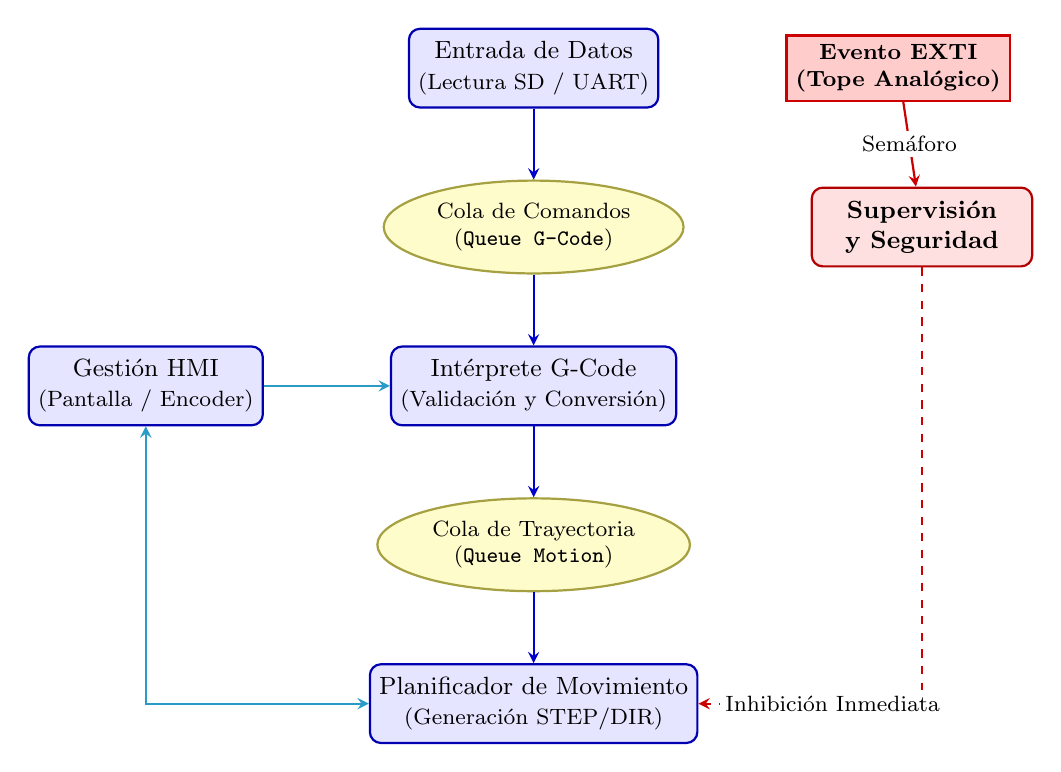
\begin{tikzpicture}[
  >=stealth, thick,
  font=\small,
  node distance=1.1cm and 1.6cm,
  task/.style={draw=blue!70!black, fill=blue!10, rectangle, rounded corners=4pt, minimum height=1.0cm, minimum width=2.8cm, align=center},
  queue/.style={draw=yellow!60!black, fill=yellow!20, ellipse, minimum height=0.8cm, minimum width=2.4cm, align=center, font=\footnotesize},
  safety/.style={draw=red!70!black, fill=red!12, rectangle, rounded corners=4pt, minimum height=1.0cm, minimum width=2.8cm, align=center, font=\small\bfseries},
  isr/.style={draw=red!80!black, fill=red!20, rectangle, minimum height=0.8cm, minimum width=2.4cm, align=center, font=\footnotesize\bfseries}
]

  % Columna Central: Pipeline de Ejecución de Mecanizado
  \node[task] (storage) {Entrada de Datos\\{\footnotesize (Lectura SD / UART)}};
  \node[queue, below=0.9cm of storage] (qcode) {Cola de Comandos\\{\footnotesize (\texttt{Queue G-Code})}};
  \node[task, below=0.9cm of qcode] (parser) {Intérprete G-Code\\{\footnotesize (Validación y Conversión)}};
  \node[queue, below=0.9cm of parser] (qmotion) {Cola de Trayectoria\\{\footnotesize (\texttt{Queue Motion})}};
  \node[task, below=0.9cm of qmotion] (planner) {Planificador de Movimiento\\{\footnotesize (Generación STEP/DIR)}};

  % Columna Izquierda: Interfaz de Usuario
  \node[task, left=of parser] (hmi) {Gestión HMI\\{\footnotesize (Pantalla / Encoder)}};

  % Columna Derecha: Sistema de Seguridad
  \node[isr, right=of storage] (exti) {Evento EXTI\\{\footnotesize (Tope Analógico)}};
  \node[safety, right=of qcode] (safetytask) {Supervisión\\y Seguridad};

  % Conexiones del Pipeline Central
  \draw[->, draw=blue!80!black] (storage) -- (qcode);
  \draw[->, draw=blue!80!black] (qcode) -- (parser);
  \draw[->, draw=blue!80!black] (parser) -- (qmotion);
  \draw[->, draw=blue!80!black] (qmotion) -- (planner);

  % Conexión HMI con Planificador y Parser
  \draw[<->, draw=cyan!80!black] (hmi) |- (planner);
  \draw[->, draw=cyan!80!black] (hmi) -- (parser);

  % Conexiones de Seguridad
  \draw[->, draw=red!80!black] (exti) -- node[midway, fill=white, inner sep=2pt, font=\footnotesize] {Semáforo} (safetytask);
  \draw[->, dashed, draw=red!80!black] (safetytask) |- node[pos=0.7, fill=white, inner sep=2pt, font=\footnotesize] {Inhibición Inmediata} (planner);

\end{tikzpicture}
}
  \caption{Esquema de arquitectura de software en tiempo real con separación por capas de prioridad y mecanismos de sincronización.}
  \label{fig.ej3:arquitectura_freertos}
\end{figure}

\section{Módulo Intérprete de Código G y Perfilado de Movimiento}
\label{sec:td2_gcode}

El sistema embebido incorporará un módulo analizador sintáctico para interpretar instrucciones normalizadas según el
estándar ISO 6983 / RS-274D. La implementación se enfocará en un subconjunto fundamental que comprende:
\begin{itemize}
  \item Movimientos de posicionamiento rápido no interpolado.
  \item Interpolación lineal con velocidad de avance controlada (\textit{feedrate}).
  \item Comandos de temporización y pausas programadas.
  \item Comandos auxiliares de control de herramientas (encendido, apagado y ajuste de velocidad del \textit{spindle}).
\end{itemize}

En la figura~\ref{fig.ej3:flujo_gcode} se describe el flujo general de datos desde la recepción de la instrucción hasta
su ejecución en los actuadores.

\begin{figure}[!ht]
  \centering
  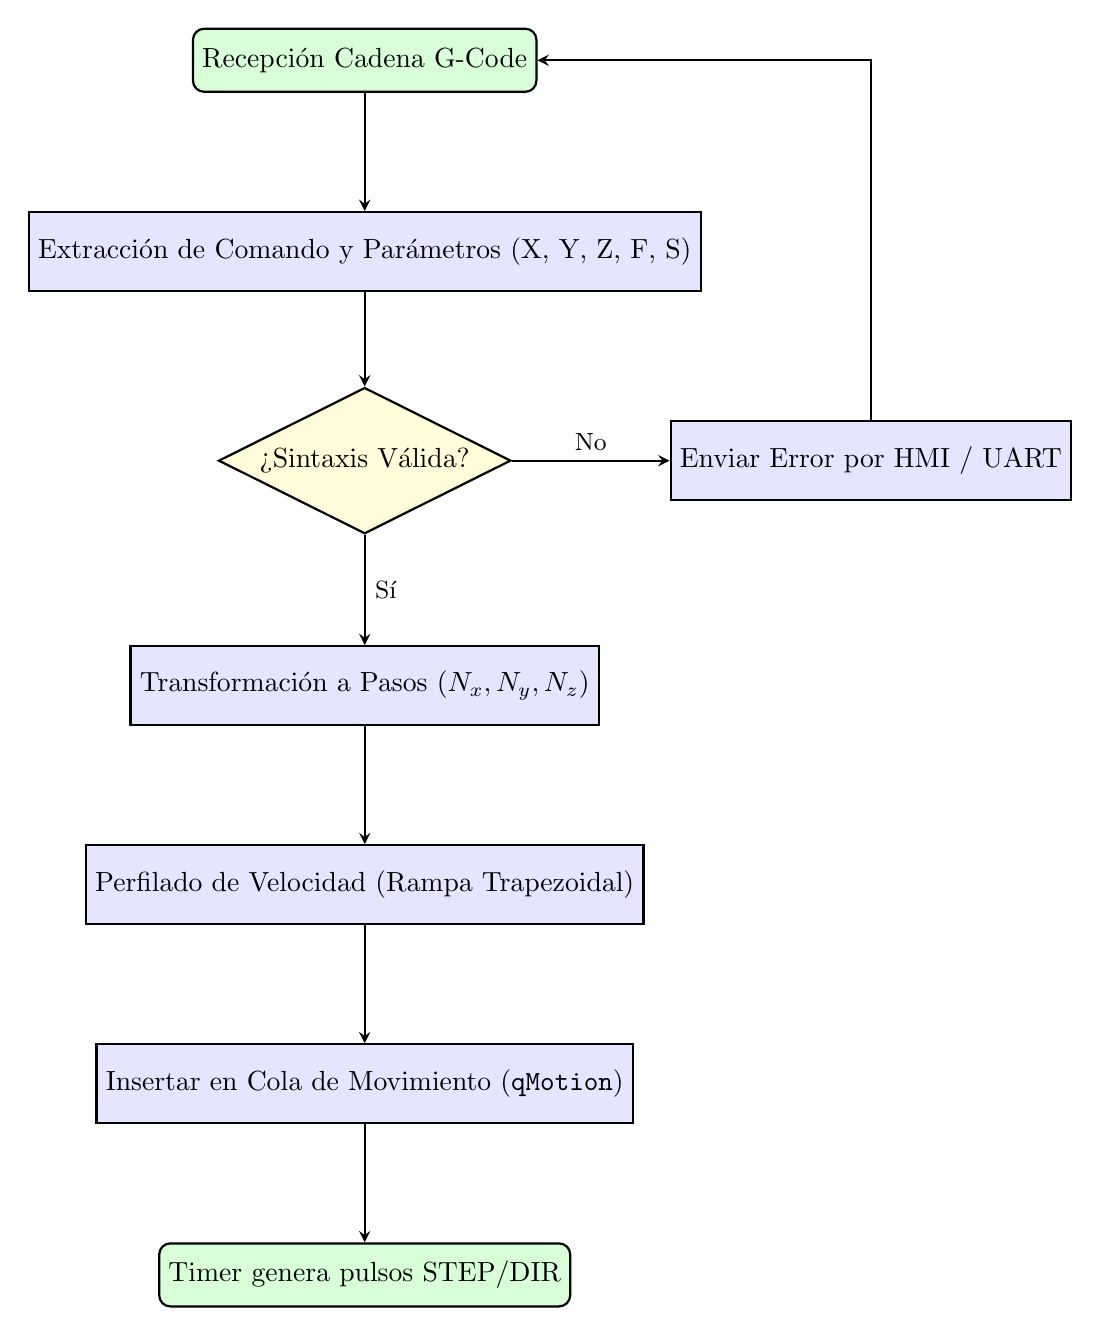
\begin{tikzpicture}[node distance=1.5cm, auto, >=stealth, thick,
  startstop/.style={draw, fill=green!15, rectangle, rounded corners, minimum height=0.8cm, text centered, align=center},
  process/.style={draw, fill=blue!10, rectangle, minimum height=1.0cm, text centered, align=center},
  decision/.style={draw, fill=yellow!15, diamond, aspect=2, inner sep=2pt, text centered, align=center}]

  \node [startstop] (start) {Recepción Cadena G-Code};
  \node [process, below=of start] (parse) {Extracción de Comando y Parámetros (X, Y, Z, F, S)};
  \node [decision, below=1.2cm of parse] (valid) {¿Sintaxis Válida?};
  \node [process, right=2.0cm of valid] (error) {Enviar Error por HMI / UART};
  \node [process, below=1.4cm of valid] (calc) {Transformación a Pasos ($N_x, N_y, N_z$)};
  \node [process, below=of calc] (plan) {Perfilado de Velocidad (Rampa Trapezoidal)};
  \node [process, below=of plan] (enqueue) {Insertar en Cola de Movimiento (\texttt{qMotion})};
  \node [startstop, below=of enqueue] (exec) {Timer genera pulsos STEP/DIR};

  \draw [->] (start) -- (parse);
  \draw [->] (parse) -- (valid);
  \draw [->] (valid) -- node[above, font=\small] {No} (error);
  \draw [->] (valid) -- node[right, font=\small] {Sí} (calc);
  \draw [->] (calc) -- (plan);
  \draw [->] (plan) -- (enqueue);
  \draw [->] (enqueue) -- (exec);
  \draw [->] (error.north) |- (start.east);
\end{tikzpicture}

  \caption{Diagrama de flujo para el procesamiento, validación y ejecución de comandos de mecanizado.}
  \label{fig.ej3:flujo_gcode}
\end{figure}

\section{Selección del Microcontrolador y Asignación de Periféricos}
\label{sec:td2_perifericos}

Como unidad central de procesamiento se utilizará un microcontrolador reciclado \textbf{GD32F103RCT6} (arquitectura ARM Cortex-M3), un reemplazo directo compatible con el STM32F103RCT6 capaz de operar a una frecuencia máxima de reloj de \SI{108}{\mega\hertz}. Al pertenecer a la misma familia de microcontroladores que la plataforma base recomendada por la cátedra (Blue Pill / STM32F103C8T6), se garantiza plena compatibilidad a nivel de arquitectura, periféricos, bibliotecas CMSIS y soporte del kernel FreeRTOS. Adicionalmente, la adopción de este componente reutilizado en encapsulado LQFP64 responde a la necesidad de contar con un adecuado margen de reserva (\textit{headroom}) de líneas de entrada/salida y temporizadores por hardware, previniendo restricciones de conectividad al definir la cantidad final de pines requeridos para los controladores de movimiento (motores paso a paso), el accionamiento del \textit{spindle}, los canales de sensado analógico y la interfaz HMI.

Para satisfacer las demandas del sistema, el dispositivo asignará el siguiente conjunto de capacidades periféricas:

\begin{itemize}
  \item \textbf{Temporizadores por Hardware (Timers):} Módulos de temporización con capacidad de interrupción periódica
    y modulación PWM para la generación determinística de frecuencias de paso y control del \textit{spindle} sin sobrecargar la CPU.
  \item \textbf{Buses de Comunicación Serie:} Interfaces sincrónicas de alta velocidad (como SPI/SDIO) para el acceso al
    almacenamiento masivo (tarjeta SD) e interfaces serie (como UART o I2C) para comunicación y periféricos de HMI.
  \item \textbf{Canales de Conversión A/D (ADC):} Lectura periódica de las tensiones provenientes del acondicionamiento analógico
    para el seguimiento del consumo energético, estado de carga y sensado de corriente.
  \item \textbf{Líneas GPIO e Interrupciones Externas (EXTI):} Control de señales de habilitación de drivers y captura
    inmediata de eventos asíncronos de seguridad.
\end{itemize}

\chapter{Máquinas e Instalaciones Eléctricas: Controladores de Potencia y Accionamientos}
\label{sec:maquinas_e_instalaciones_electricas}

En la asignatura Máquinas e Instalaciones Eléctricas, el anteproyecto desarrolla el diseño electromecánico y de
potencia para los accionamientos de la CNC. Esto abarca los controladores modulares de velocidad y sentido de giro para
los motores paso a paso de los tres ejes y el regulador de potencia para la herramienta de corte (motor DC).

\section{Requerimiento de Diseño Modular por Canal}
\label{sec:myie_modularidad}

Para garantizar un mantenimiento sencillo, una escalabilidad flexible y cumplir con la consigna académica, el sistema
de potencia adopta una topología estrictamente modular.

Cada eje mecánico (X, Y, Z) cuenta con su propio módulo electrónico independiente montado en una tarjeta PCB canalizada.
Cada canal de potencia integra:
\begin{itemize}
  \item La etapa lógica de decodificación de las señales digitales STEP y DIR.
  \item Las etapas de potencia compuestas por puentes H para la conmutación de las fases del motor paso a paso.
  \item La resistencia de derivación ($R_{shunt\_canal}$) colocada en el retorno de masa común del canal, a fin de permitir
    que la etapa analógica de Electrónica Aplicada II tome la medición de corriente total consumida por dicho canal.
\end{itemize}

En la figura~\ref{crkt.ej4:driver_paso_a_paso} se presenta la estructura de bloques de un canal modular de potencia.

\begin{figure}[!ht]
  \centering
  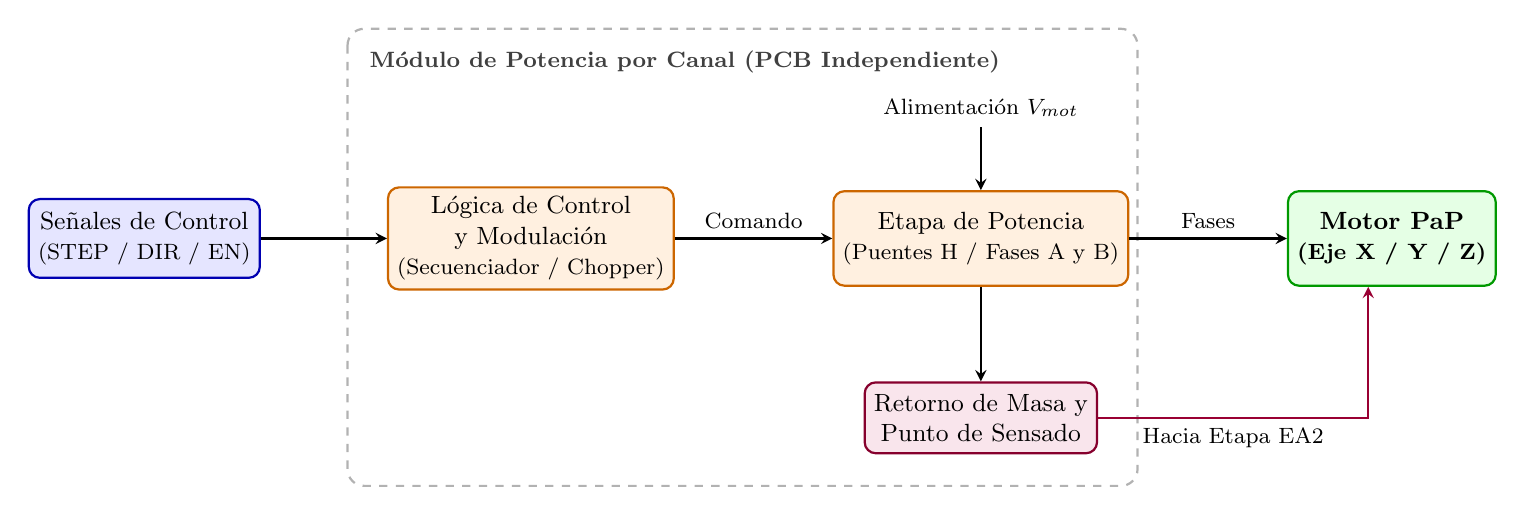
\begin{tikzpicture}[
  >=stealth, thick,
  font=\small,
  node distance=1.2cm and 2.0cm,
  block/.style={draw=orange!80!black, fill=orange!12, rectangle, rounded corners=4pt, minimum height=1.2cm, minimum width=2.9cm, align=center},
  ctrl/.style={draw=blue!70!black, fill=blue!10, rectangle, rounded corners=4pt, minimum height=1.0cm, minimum width=2.5cm, align=center},
  sens/.style={draw=purple!70!black, fill=purple!10, rectangle, rounded corners=4pt, minimum height=0.9cm, minimum width=2.9cm, align=center},
  motor/.style={draw=green!60!black, fill=green!10, rectangle, rounded corners=4pt, minimum height=1.2cm, minimum width=2.6cm, align=center, font=\small\bfseries}
]

  % Bloques principales
  \node[ctrl] (ctrl) {Señales de Control\\{\footnotesize (STEP / DIR / EN)}};
  \node[block, right=1.6cm of ctrl] (logic) {Lógica de Control\\y Modulación\\{\footnotesize (Secuenciador / Chopper)}};
  \node[block, right=2.0cm of logic] (power) {Etapa de Potencia\\{\footnotesize (Puentes H / Fases A y B)}};
  \node[sens, below=1.2cm of power] (sens) {Retorno de Masa y\\Punto de Sensado};
  \node[motor, right=2.0cm of power] (motor) {Motor PaP\\{\footnotesize (Eje X / Y / Z)}};

  % Contenedor Modular (Caja con margen superior amplio de 1.8cm para no colisionar con la alimentación)
  \draw[dashed, draw=gray!60, rounded corners=6pt] 
    ([xshift=-0.5cm, yshift=2.0cm]logic.north west) rectangle 
    ([xshift=0.5cm, yshift=-0.4cm]sens.south east);
  \node[anchor=north west, font=\footnotesize\bfseries\color{black!75}] 
    at ([xshift=-0.35cm, yshift=1.85cm]logic.north west) {Módulo de Potencia por Canal (PCB Independiente)};

  % Conexiones con etiquetas centradas
  \draw[->] (ctrl) -- (logic);
  \draw[->] (logic) -- node[above, font=\footnotesize] {Comando} (power);
  \draw[->] (power) -- node[above, font=\footnotesize] {Fases} (motor);
  \draw[->] (power) -- (sens);
  \draw[->, draw=purple!80!black] (sens.east) -| node[pos=0.25, below, font=\footnotesize] {Hacia Etapa EA2} ([xshift=-0.3cm]motor.south);

  % Alimentación con espacio holgado
  \draw[<-] (power.north) -- ++(0,0.8) node[above, font=\footnotesize] {Alimentación $V_{mot}$};

\end{tikzpicture}

  \caption{Diagrama de bloques funcional de un canal modular de potencia para motor paso a paso.}
  \label{crkt.ej4:driver_paso_a_paso}
\end{figure}

\section{Controlador de Motores Paso a Paso y Pasos Fraccionados (Micropasos)}
\label{sec:myie_paso_a_paso}

Los motores paso a paso recuperados de las impresoras suelen ser del tipo bipolar de dos fases. El controlador del
canal genera las secuencias de activación necesarias mediante las señales de entrada:
\begin{itemize}
  \item \textbf{Señal STEP:} Cada flanco de subida de esta señal determina el avance de un paso (o subpaso) angular del
    motor. La frecuencia de la señal impone directamente la velocidad de rotación ($n$ en $\mathrm{rpm}$).
  \item \textbf{Señal DIR:} Define la secuencia de fase aplicada al motor, determinando si el giro se realiza en sentido
    horario o antihorario.
\end{itemize}

\subsection{Evaluación de Complejidad para Pasos Fraccionados}
Un aspecto central de estudio en la materia es el análisis de implementar modulación por troceado de corriente
(\textit{chopping PWM}) para lograr pasos fraccionados (micropasos de 1/2, 1/4 o 1/8). 

En un accionamiento por pasos completos, la conmutación abrupta de tensión genera vibraciones y resonancia en la
estructura liviana de la impresora. La implementación de micropasos aproxima la corriente en las fases a ondas senoidales
desfasadas $90^\circ$, tal como se expresa en la ecuación~\ref{eq.ej4:fases_micro}:

\begin{equation}
  I_A(\theta) = I_{max} \cdot \sin(\theta), \quad I_B(\theta) = I_{max} \cdot \cos(\theta)
  \label{eq.ej4:fases_micro}
\end{equation}

El anteproyecto plantea la evaluación de complejidad para determinar si se utilizará control analógico por chopper
dedicado o generación de consigna sinusoidal desde el microcontrolador, ponderando el compromiso entre suavidad de
movimiento, torque disponible y tiempo de desarrollo.

\section{Controlador del Motor DC para el Spindle (Fresa)}
\label{sec:myie_spindle}

El cabezal de mecanizado utiliza un motor de corriente continua de alta velocidad para impulsar la fresa o mecha. La
regulación de su velocidad resulta indispensable para adaptar las condiciones de corte al material trabajado.

El circuito de potencia utiliza un MOSFET de potencia actuando como conmutador de estado sólido en serie con la carga,
controlado por una señal PWM generada desde la placa digital. La figura~\ref{crkt.ej4:driver_spindle} muestra el
esquema circuital de la etapa de potencia del motor DC.

\begin{figure}[!ht]
  \centering
  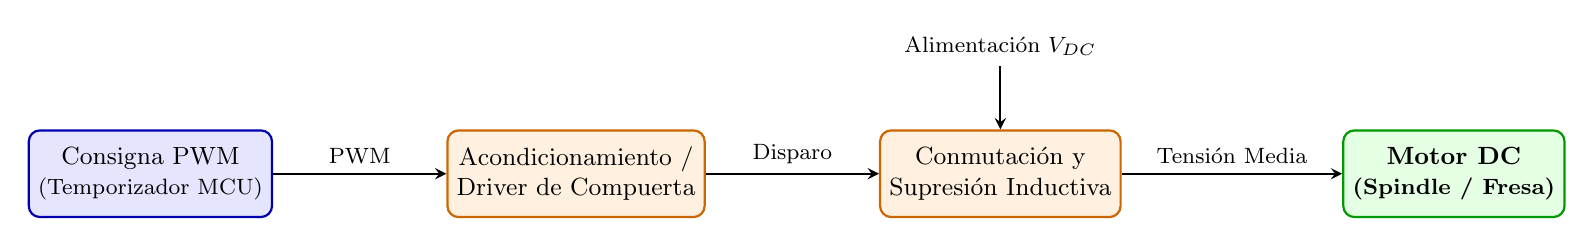
\begin{tikzpicture}[
  >=stealth, thick,
  font=\small,
  node distance=1.0cm and 2.2cm,
  ctrl/.style={draw=blue!70!black, fill=blue!10, rectangle, rounded corners=4pt, minimum height=1.1cm, minimum width=2.6cm, align=center},
  block/.style={draw=orange!80!black, fill=orange!12, rectangle, rounded corners=4pt, minimum height=1.1cm, minimum width=2.8cm, align=center},
  motor/.style={draw=green!60!black, fill=green!10, rectangle, rounded corners=4pt, minimum height=1.1cm, minimum width=2.6cm, align=center, font=\small\bfseries}
]

  \node[ctrl] (ctrl) {Consigna PWM\\{\footnotesize (Temporizador MCU)}};
  \node[block, right=2.2cm of ctrl] (driver) {Acondicionamiento /\\Driver de Compuerta};
  \node[block, right=2.2cm of driver] (switch) {Conmutación y\\Supresión Inductiva};
  \node[motor, right=2.8cm of switch] (motor) {Motor DC\\{\footnotesize (Spindle / Fresa)}};

  % Conexiones lineales con espacio amplio para las etiquetas
  \draw[->] (ctrl) -- node[above, font=\footnotesize] {PWM} (driver);
  \draw[->] (driver) -- node[above, font=\footnotesize] {Disparo} (switch);
  \draw[->] (switch) -- node[above, font=\footnotesize] {Tensión Media} (motor);

  % Alimentación de potencia
  \draw[<-] (switch.north) -- ++(0,0.8) node[above, font=\footnotesize] {Alimentación $V_{DC}$};

\end{tikzpicture}

  \caption{Esquema circuital de accionamiento de potencia PWM para el motor DC de la herramienta de corte.}
  \label{crkt.ej4:driver_spindle}
\end{figure}

El diodo en paralelo inverso con la inductancia del motor (\textit{flyback diode}) protege al transistor de sobretensiones
inductivas provocadas por el apagado rápido del MOSFET durante la conmutación PWM. La velocidad del motor responde de forma
directamente proporcional al ciclo de trabajo ($\delta$) de la señal de control.

\chapter{Conclusiones y Plan de Trabajo}
\label{sec:conclusiones}

El anteproyecto presentado demuestra la viabilidad técnica y metodológica de construir una máquina de control numérico
computarizado de bajo costo reutilizando componentes electromecánicos de impresoras fuera de uso, al tiempo que integra
de manera armónica los contenidos teóricos y prácticos de tres asignaturas troncales del cuarto año de Ingeniería
Electrónica.

\section{Resumen de Integración Técnica}
\label{sec:resumen_integracion}

La tabla~\ref{tab.ej5:resumen_materias} sintetiza la distribución de responsabilidades técnicas e hitos de diseño por
asignatura.

\begin{table}[!ht]
  \centering
  \resizebox{\textwidth}{!}{
    \begin{tabular}{|l|p{6cm}|p{6cm}|}
      \hline
      \textbf{Asignatura} & \textbf{Módulo del Proyecto} & \textbf{Conceptos Clave Aplicados} \\ \hline
      Electrónica Aplicada II & Sensado de corriente y final de carrera electrónico & Amplificador diferencial, amplificador operacional, filtro RC, comparador con histéresis (Schmitt trigger), acondicionamiento analógico. \\ \hline
      Técnicas Digitales II & Controlador central embebido e interfaz HMI & RTOS (FreeRTOS), interpretador de código G, buses SPI e I2C, conversor ADC, interrupciones externas EXTI, timers por hardware. \\ \hline
      Máquinas e Inst. Eléctricas & Controladores modulares de motores PaP y Spindle & Motores paso a paso bipolares, control modular por canal, modulación PWM, puentes H, diodo flyback, evaluación de micropasos. \\ \hline
    \end{tabular}
  }
  \caption{Matriz de integración conceptual por asignatura académica.}
  \label{tab.ej5:resumen_materias}
\end{table}

\section{Pasos Futuros para la Etapa de Desarrollo Final}
\label{sec:pasos_futuros}

Con la aprobación del presente anteproyecto, el equipo de trabajo avanzará en las siguientes etapas del proyecto final:
\begin{enumerate}
  \item Caracterización mecánica del chasis de impresora recuperado y selección final de motores.
  \item Simulación analógica en LTSpice de la etapa de sensado con OpAmps y comparador de Electrónica Aplicada II.
  \item Diseño de los esquemáticos y trazado de placas de circuito impreso (PCB) en KiCad para los controladores modulares
    de potencia.
  \item Desarrollo del firmware embebido sobre FreeRTOS en lenguaje C/C++ verificando tiempos de ejecución y latencias.
  \item Ensamble, calibración y pruebas de mecanizado real sobre placas de circuito impreso y materiales de prueba.
\end{enumerate}


\nocite{*}
\printbibliography[heading=bibnumbered, title={Fuentes}]

\end{document}
